\documentclass[]{article}
\usepackage{lmodern}
\usepackage{amssymb,amsmath}
\usepackage{ifxetex,ifluatex}
\usepackage{fixltx2e} % provides \textsubscript
\ifnum 0\ifxetex 1\fi\ifluatex 1\fi=0 % if pdftex
  \usepackage[T1]{fontenc}
  \usepackage[utf8]{inputenc}
\else % if luatex or xelatex
  \ifxetex
    \usepackage{mathspec}
  \else
    \usepackage{fontspec}
  \fi
  \defaultfontfeatures{Ligatures=TeX,Scale=MatchLowercase}
\fi
% use upquote if available, for straight quotes in verbatim environments
\IfFileExists{upquote.sty}{\usepackage{upquote}}{}
% use microtype if available
\IfFileExists{microtype.sty}{%
\usepackage{microtype}
\UseMicrotypeSet[protrusion]{basicmath} % disable protrusion for tt fonts
}{}
\usepackage[margin=1in]{geometry}
\usepackage{hyperref}
\hypersetup{unicode=true,
            pdftitle={Assignment 7 Coding Part},
            pdfauthor={Kaicheng Luo},
            pdfborder={0 0 0},
            breaklinks=true}
\urlstyle{same}  % don't use monospace font for urls
\usepackage{color}
\usepackage{fancyvrb}
\newcommand{\VerbBar}{|}
\newcommand{\VERB}{\Verb[commandchars=\\\{\}]}
\DefineVerbatimEnvironment{Highlighting}{Verbatim}{commandchars=\\\{\}}
% Add ',fontsize=\small' for more characters per line
\usepackage{framed}
\definecolor{shadecolor}{RGB}{248,248,248}
\newenvironment{Shaded}{\begin{snugshade}}{\end{snugshade}}
\newcommand{\KeywordTok}[1]{\textcolor[rgb]{0.13,0.29,0.53}{\textbf{#1}}}
\newcommand{\DataTypeTok}[1]{\textcolor[rgb]{0.13,0.29,0.53}{#1}}
\newcommand{\DecValTok}[1]{\textcolor[rgb]{0.00,0.00,0.81}{#1}}
\newcommand{\BaseNTok}[1]{\textcolor[rgb]{0.00,0.00,0.81}{#1}}
\newcommand{\FloatTok}[1]{\textcolor[rgb]{0.00,0.00,0.81}{#1}}
\newcommand{\ConstantTok}[1]{\textcolor[rgb]{0.00,0.00,0.00}{#1}}
\newcommand{\CharTok}[1]{\textcolor[rgb]{0.31,0.60,0.02}{#1}}
\newcommand{\SpecialCharTok}[1]{\textcolor[rgb]{0.00,0.00,0.00}{#1}}
\newcommand{\StringTok}[1]{\textcolor[rgb]{0.31,0.60,0.02}{#1}}
\newcommand{\VerbatimStringTok}[1]{\textcolor[rgb]{0.31,0.60,0.02}{#1}}
\newcommand{\SpecialStringTok}[1]{\textcolor[rgb]{0.31,0.60,0.02}{#1}}
\newcommand{\ImportTok}[1]{#1}
\newcommand{\CommentTok}[1]{\textcolor[rgb]{0.56,0.35,0.01}{\textit{#1}}}
\newcommand{\DocumentationTok}[1]{\textcolor[rgb]{0.56,0.35,0.01}{\textbf{\textit{#1}}}}
\newcommand{\AnnotationTok}[1]{\textcolor[rgb]{0.56,0.35,0.01}{\textbf{\textit{#1}}}}
\newcommand{\CommentVarTok}[1]{\textcolor[rgb]{0.56,0.35,0.01}{\textbf{\textit{#1}}}}
\newcommand{\OtherTok}[1]{\textcolor[rgb]{0.56,0.35,0.01}{#1}}
\newcommand{\FunctionTok}[1]{\textcolor[rgb]{0.00,0.00,0.00}{#1}}
\newcommand{\VariableTok}[1]{\textcolor[rgb]{0.00,0.00,0.00}{#1}}
\newcommand{\ControlFlowTok}[1]{\textcolor[rgb]{0.13,0.29,0.53}{\textbf{#1}}}
\newcommand{\OperatorTok}[1]{\textcolor[rgb]{0.81,0.36,0.00}{\textbf{#1}}}
\newcommand{\BuiltInTok}[1]{#1}
\newcommand{\ExtensionTok}[1]{#1}
\newcommand{\PreprocessorTok}[1]{\textcolor[rgb]{0.56,0.35,0.01}{\textit{#1}}}
\newcommand{\AttributeTok}[1]{\textcolor[rgb]{0.77,0.63,0.00}{#1}}
\newcommand{\RegionMarkerTok}[1]{#1}
\newcommand{\InformationTok}[1]{\textcolor[rgb]{0.56,0.35,0.01}{\textbf{\textit{#1}}}}
\newcommand{\WarningTok}[1]{\textcolor[rgb]{0.56,0.35,0.01}{\textbf{\textit{#1}}}}
\newcommand{\AlertTok}[1]{\textcolor[rgb]{0.94,0.16,0.16}{#1}}
\newcommand{\ErrorTok}[1]{\textcolor[rgb]{0.64,0.00,0.00}{\textbf{#1}}}
\newcommand{\NormalTok}[1]{#1}
\usepackage{graphicx,grffile}
\makeatletter
\def\maxwidth{\ifdim\Gin@nat@width>\linewidth\linewidth\else\Gin@nat@width\fi}
\def\maxheight{\ifdim\Gin@nat@height>\textheight\textheight\else\Gin@nat@height\fi}
\makeatother
% Scale images if necessary, so that they will not overflow the page
% margins by default, and it is still possible to overwrite the defaults
% using explicit options in \includegraphics[width, height, ...]{}
\setkeys{Gin}{width=\maxwidth,height=\maxheight,keepaspectratio}
\IfFileExists{parskip.sty}{%
\usepackage{parskip}
}{% else
\setlength{\parindent}{0pt}
\setlength{\parskip}{6pt plus 2pt minus 1pt}
}
\setlength{\emergencystretch}{3em}  % prevent overfull lines
\providecommand{\tightlist}{%
  \setlength{\itemsep}{0pt}\setlength{\parskip}{0pt}}
\setcounter{secnumdepth}{0}
% Redefines (sub)paragraphs to behave more like sections
\ifx\paragraph\undefined\else
\let\oldparagraph\paragraph
\renewcommand{\paragraph}[1]{\oldparagraph{#1}\mbox{}}
\fi
\ifx\subparagraph\undefined\else
\let\oldsubparagraph\subparagraph
\renewcommand{\subparagraph}[1]{\oldsubparagraph{#1}\mbox{}}
\fi

%%% Use protect on footnotes to avoid problems with footnotes in titles
\let\rmarkdownfootnote\footnote%
\def\footnote{\protect\rmarkdownfootnote}

%%% Change title format to be more compact
\usepackage{titling}

% Create subtitle command for use in maketitle
\providecommand{\subtitle}[1]{
  \posttitle{
    \begin{center}\large#1\end{center}
    }
}

\setlength{\droptitle}{-2em}

  \title{Assignment 7 Coding Part}
    \pretitle{\vspace{\droptitle}\centering\huge}
  \posttitle{\par}
    \author{Kaicheng Luo}
    \preauthor{\centering\large\emph}
  \postauthor{\par}
      \predate{\centering\large\emph}
  \postdate{\par}
    \date{2019/10/29}


\begin{document}
\maketitle

\begin{Shaded}
\begin{Highlighting}[]
\NormalTok{d <-}\StringTok{ }\ControlFlowTok{function}\NormalTok{(x,z,}\DataTypeTok{p=}\DecValTok{2}\NormalTok{)\{}
  \KeywordTok{return}\NormalTok{((}\KeywordTok{abs}\NormalTok{(x}\OperatorTok{-}\NormalTok{z)}\OperatorTok{^}\NormalTok{p)}\OperatorTok{^}\NormalTok{(}\DecValTok{1}\OperatorTok{/}\NormalTok{p))}
\NormalTok{\}}

\NormalTok{kNNW <-}\StringTok{ }\ControlFlowTok{function}\NormalTok{(x,y,z,k,p)\{}
\NormalTok{  result =}\StringTok{ }\KeywordTok{c}\NormalTok{()}
  \ControlFlowTok{for}\NormalTok{ (query }\ControlFlowTok{in} \DecValTok{1}\OperatorTok{:}\KeywordTok{length}\NormalTok{(z))}
\NormalTok{  \{}
    \CommentTok{# First, find the nearest k points}
\NormalTok{    indices <-}\StringTok{ }\KeywordTok{which}\NormalTok{(}\KeywordTok{rank}\NormalTok{(}\KeywordTok{d}\NormalTok{(x,z[query],p))}\OperatorTok{<=}\NormalTok{k)}
    \CommentTok{# Access the value and feature of those k points}
\NormalTok{    label <-}\StringTok{ }\NormalTok{y[indices]}
\NormalTok{    feature <-}\StringTok{ }\NormalTok{x[indices]}
\NormalTok{    pred =}\StringTok{ }\DecValTok{0}
\NormalTok{    denominator =}\StringTok{ }\DecValTok{0}
    \CommentTok{# Calculate the weights}
    \ControlFlowTok{for}\NormalTok{ (i }\ControlFlowTok{in} \DecValTok{1}\OperatorTok{:}\KeywordTok{length}\NormalTok{(label))\{}
\NormalTok{      denominator =}\StringTok{ }\NormalTok{denominator }\OperatorTok{+}\StringTok{ }\KeywordTok{exp}\NormalTok{(}\OperatorTok{-}\KeywordTok{d}\NormalTok{(feature[i], z[query], p))}
\NormalTok{    \}}
    \ControlFlowTok{for}\NormalTok{ (i }\ControlFlowTok{in} \DecValTok{1}\OperatorTok{:}\KeywordTok{length}\NormalTok{(label))\{}
\NormalTok{      pred =}\StringTok{ }\NormalTok{pred }\OperatorTok{+}\StringTok{ }\NormalTok{label[i]}\OperatorTok{*}\KeywordTok{exp}\NormalTok{(}\OperatorTok{-}\KeywordTok{d}\NormalTok{(feature[i], z[query], p)) }\OperatorTok{/}\StringTok{ }\NormalTok{denominator}
\NormalTok{    \}}
\NormalTok{    result =}\StringTok{ }\KeywordTok{c}\NormalTok{(result, pred)}
\NormalTok{  \}}
  \KeywordTok{return}\NormalTok{(result)}
\NormalTok{\}}

\CommentTok{# Note that in the simple scenario, L1 norm = L2 norm}
\KeywordTok{set.seed}\NormalTok{(}\DecValTok{12345}\NormalTok{)}
\NormalTok{x <-}\StringTok{ }\KeywordTok{runif}\NormalTok{(}\OperatorTok{-}\DecValTok{2}\NormalTok{, }\DecValTok{2}\NormalTok{, }\DataTypeTok{n =} \DecValTok{100}\NormalTok{) }
\NormalTok{f <-}\StringTok{ }\ControlFlowTok{function}\NormalTok{(u)\{}
  \KeywordTok{return}\NormalTok{(}\KeywordTok{sin}\NormalTok{(pi}\OperatorTok{*}\NormalTok{u) }\OperatorTok{+}\StringTok{ }\NormalTok{u}\OperatorTok{^}\DecValTok{2}\NormalTok{)}
\NormalTok{\}}
\NormalTok{y <-}\StringTok{ }\KeywordTok{f}\NormalTok{(x) }\OperatorTok{+}\StringTok{ }\KeywordTok{rnorm}\NormalTok{(}\KeywordTok{length}\NormalTok{(x), }\DataTypeTok{sd =} \FloatTok{0.2}\NormalTok{)}
\CommentTok{# # one query point, k = 10 neighbors, manhattan distance}
\CommentTok{# yhat = kNNW(x, y, z = 0, k = 10, p = 1)}
\CommentTok{# # one query point, k = 50 neighbors, manhattan distance}
\CommentTok{# yhat = kNNW(x, y, z = 0, k = 50, p = 1)}
\CommentTok{# # various query points, k = 50 neighbors, manhattan distance}
\CommentTok{# yhat = kNNW(x, y, z = c(-0.5, 0, 0.5), k = 50, p = 1)}
\end{Highlighting}
\end{Shaded}

\begin{Shaded}
\begin{Highlighting}[]
\CommentTok{# Generate some test data}
\NormalTok{z =}\StringTok{ }\KeywordTok{seq}\NormalTok{(}\OperatorTok{-}\DecValTok{2}\NormalTok{, }\DecValTok{2}\NormalTok{, }\FloatTok{0.01}\NormalTok{)}
\NormalTok{yhat =}\StringTok{ }\KeywordTok{kNNW}\NormalTok{(x, y, }\DataTypeTok{z =}\NormalTok{ z, }\DataTypeTok{k =} \DecValTok{1}\NormalTok{, }\DataTypeTok{p =} \DecValTok{1}\NormalTok{)}
\NormalTok{yreal <-}\StringTok{ }\KeywordTok{f}\NormalTok{(z) }\OperatorTok{+}\StringTok{ }\KeywordTok{rnorm}\NormalTok{(}\KeywordTok{length}\NormalTok{(z), }\DataTypeTok{sd =} \FloatTok{0.2}\NormalTok{)}
\KeywordTok{ggplot}\NormalTok{() }\OperatorTok{+}\StringTok{ }\KeywordTok{theme_bw}\NormalTok{() }\OperatorTok{+}
\StringTok{  }\KeywordTok{geom_point}\NormalTok{(}\KeywordTok{aes}\NormalTok{(}\DataTypeTok{x =}\NormalTok{ z, }\DataTypeTok{y =}\NormalTok{ yhat), }\DataTypeTok{color =} \StringTok{"maroon"}\NormalTok{)}
\end{Highlighting}
\end{Shaded}

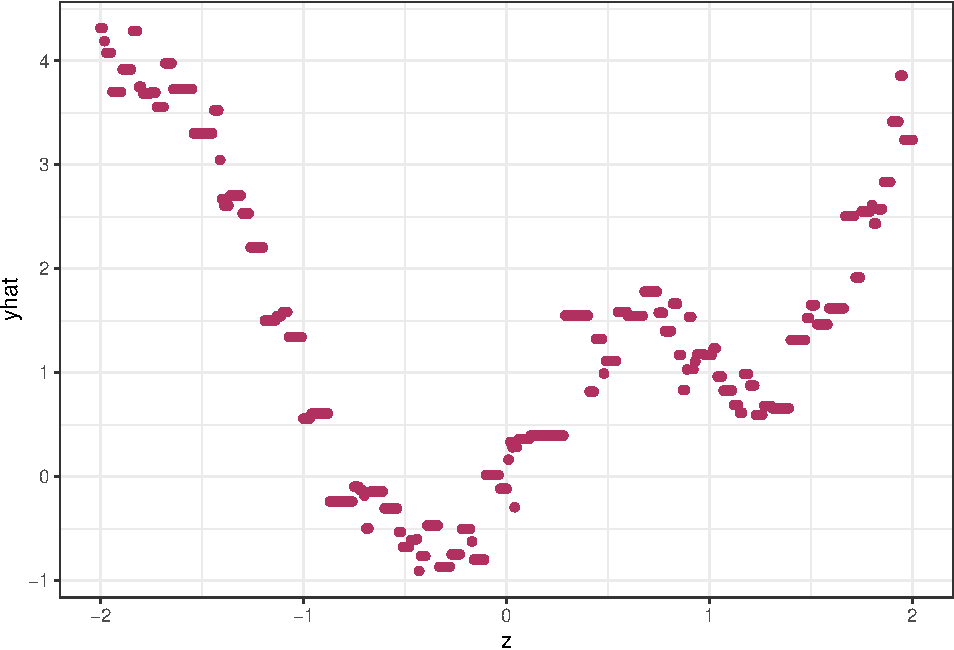
\includegraphics{hw7_files/figure-latex/unnamed-chunk-2-1.pdf}

\begin{Shaded}
\begin{Highlighting}[]
\KeywordTok{ggplot}\NormalTok{() }\OperatorTok{+}\StringTok{ }\KeywordTok{theme_bw}\NormalTok{() }\OperatorTok{+}
\StringTok{  }\KeywordTok{geom_point}\NormalTok{(}\KeywordTok{aes}\NormalTok{(}\DataTypeTok{x =}\NormalTok{ z, }\DataTypeTok{y =}\NormalTok{ yreal), }\DataTypeTok{color =} \StringTok{"maroon"}\NormalTok{)}
\end{Highlighting}
\end{Shaded}

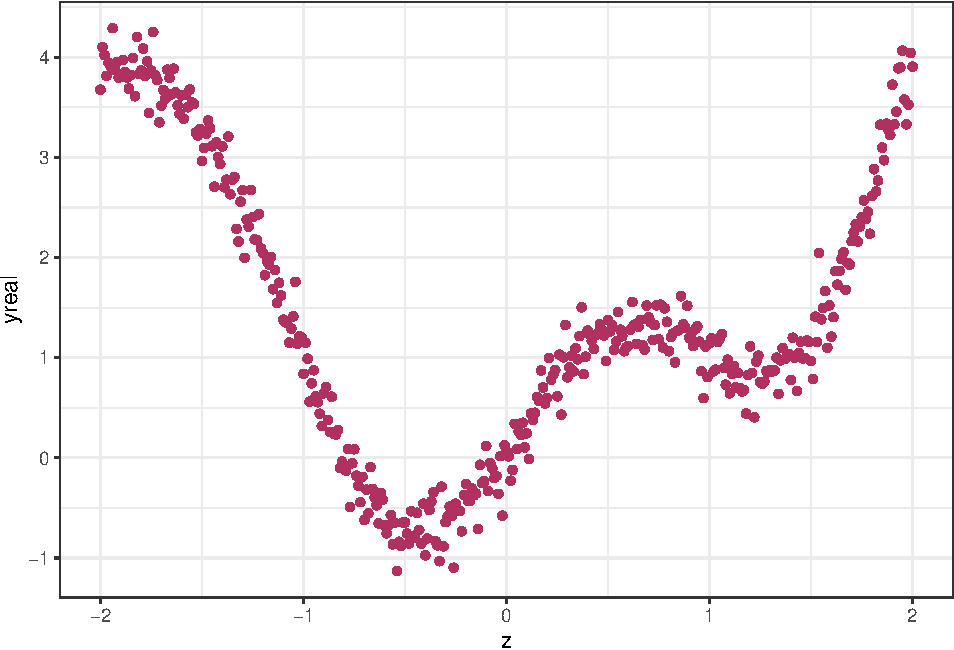
\includegraphics{hw7_files/figure-latex/unnamed-chunk-2-2.pdf}

\begin{Shaded}
\begin{Highlighting}[]
\ControlFlowTok{for}\NormalTok{ (i }\ControlFlowTok{in} \KeywordTok{c}\NormalTok{(}\DecValTok{10}\NormalTok{,}\DecValTok{30}\NormalTok{,}\DecValTok{50}\NormalTok{,}\DecValTok{70}\NormalTok{,}\DecValTok{100}\NormalTok{))\{}
\NormalTok{  yhat =}\StringTok{ }\KeywordTok{kNNW}\NormalTok{(x, y, }\DataTypeTok{z =}\NormalTok{ z, }\DataTypeTok{k =}\NormalTok{ i, }\DataTypeTok{p =} \DecValTok{1}\NormalTok{)}
  \KeywordTok{print}\NormalTok{(}\KeywordTok{ggplot}\NormalTok{() }\OperatorTok{+}\StringTok{ }\KeywordTok{theme_bw}\NormalTok{() }\OperatorTok{+}
\StringTok{    }\KeywordTok{geom_point}\NormalTok{(}\KeywordTok{aes}\NormalTok{(}\DataTypeTok{x =}\NormalTok{ z, }\DataTypeTok{y =}\NormalTok{ yhat), }\DataTypeTok{color =} \StringTok{"maroon"}\NormalTok{))}
\NormalTok{\}}
\end{Highlighting}
\end{Shaded}

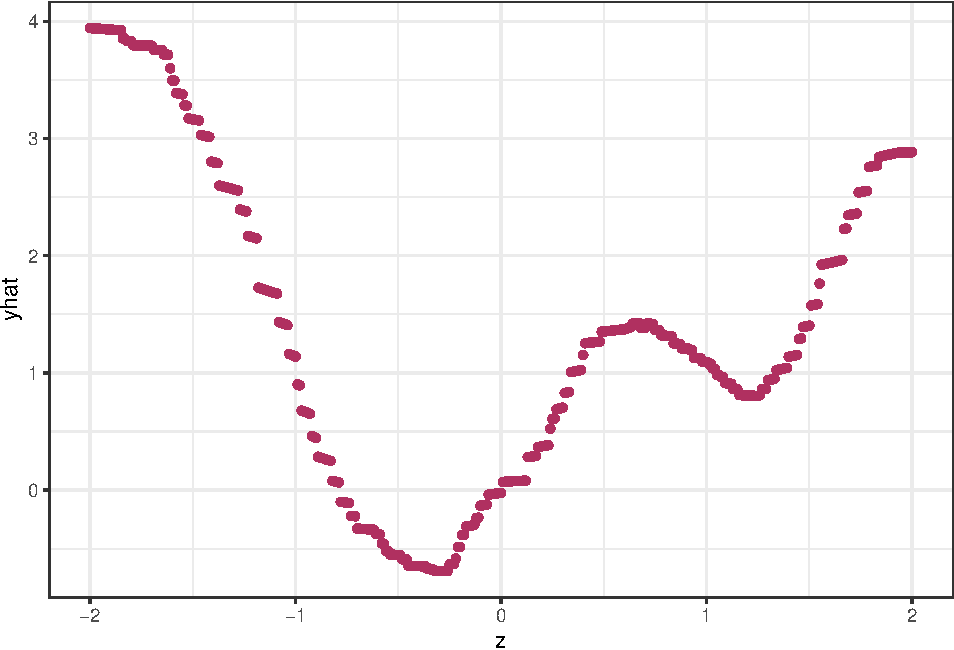
\includegraphics{hw7_files/figure-latex/unnamed-chunk-3-1.pdf}
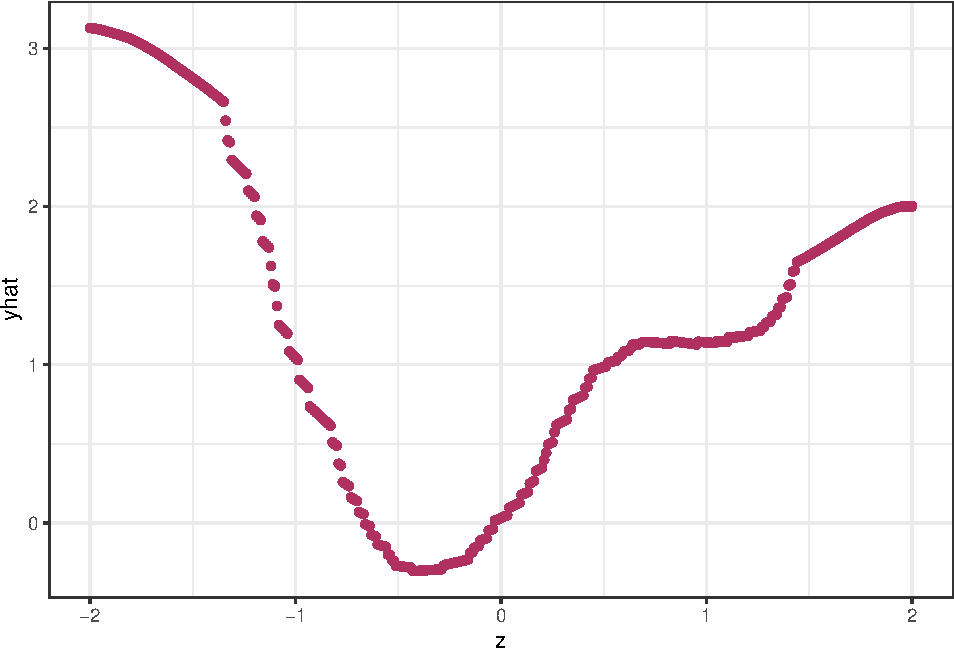
\includegraphics{hw7_files/figure-latex/unnamed-chunk-3-2.pdf}
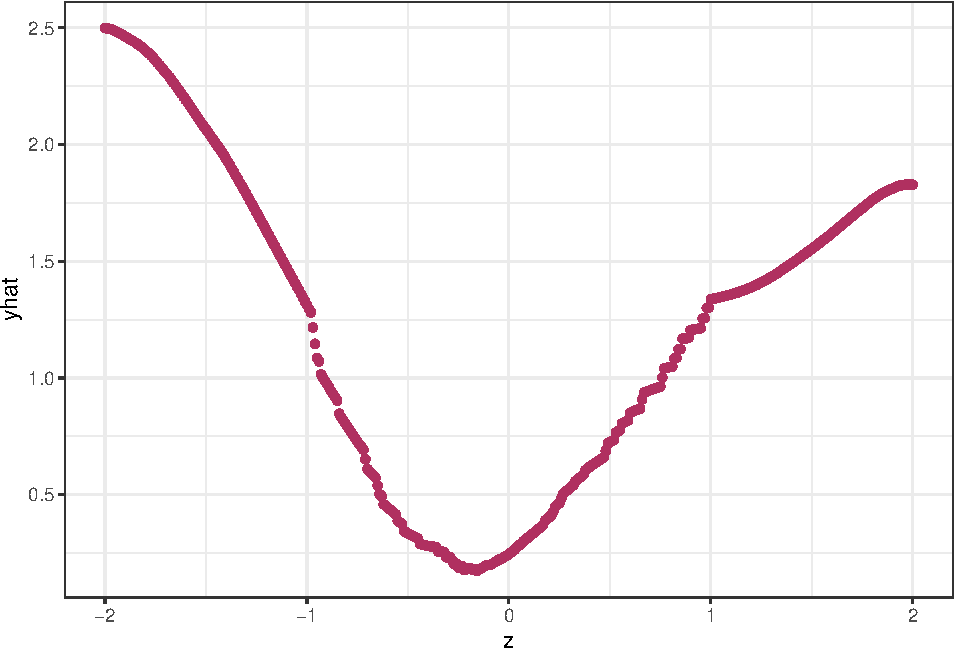
\includegraphics{hw7_files/figure-latex/unnamed-chunk-3-3.pdf}
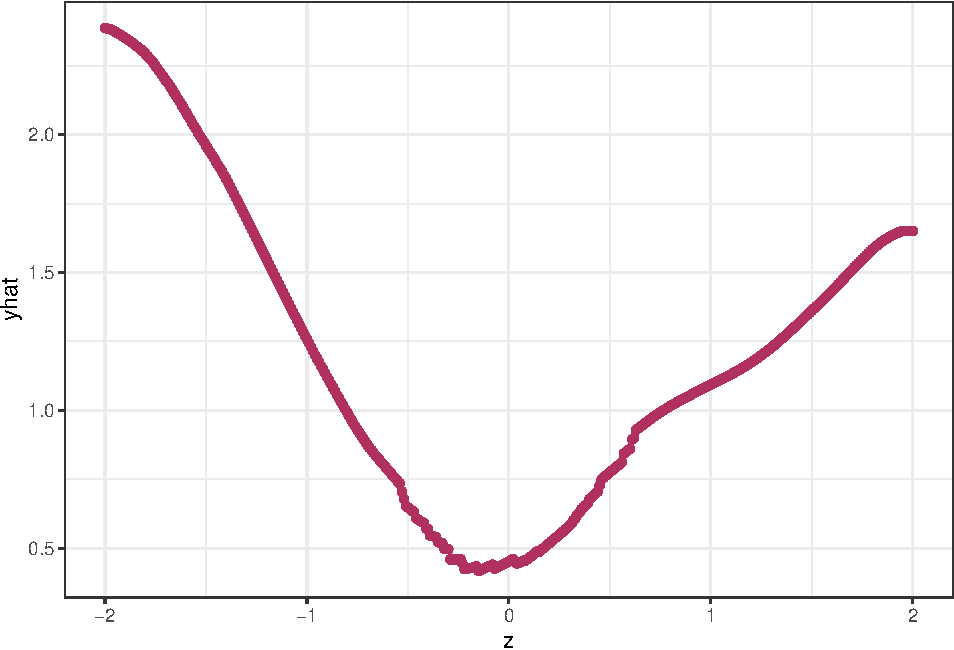
\includegraphics{hw7_files/figure-latex/unnamed-chunk-3-4.pdf}
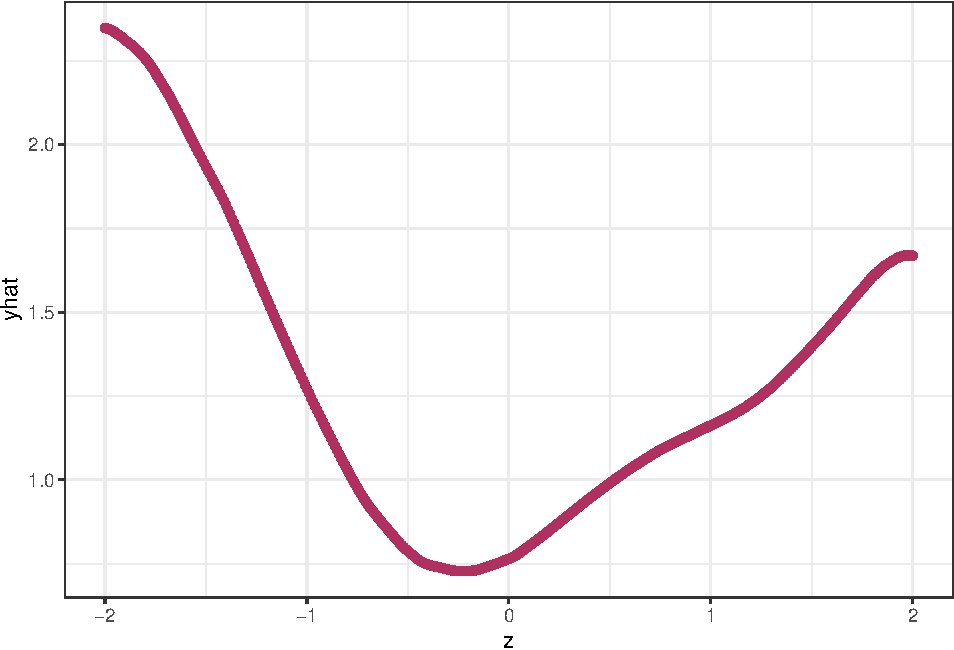
\includegraphics{hw7_files/figure-latex/unnamed-chunk-3-5.pdf}

\begin{Shaded}
\begin{Highlighting}[]
\CommentTok{# Problem 6}
\KeywordTok{data}\NormalTok{(Boston)}
\NormalTok{trainingSet <-}\StringTok{ }\NormalTok{Boston }\OperatorTok\StringTok{ }\NormalTok{dplyr}\OperatorTok{::}\KeywordTok{select}\NormalTok{(dis, nox)}
\NormalTok{x =}\StringTok{ }\NormalTok{trainingSet}\OperatorTok{$}\NormalTok{dis}
\NormalTok{y =}\StringTok{ }\NormalTok{trainingSet}\OperatorTok{$}\NormalTok{nox}
\end{Highlighting}
\end{Shaded}

\begin{Shaded}
\begin{Highlighting}[]
\CommentTok{# Q1: Fit a model with, say, degree 5}
\NormalTok{model <-}\StringTok{ }\KeywordTok{lm}\NormalTok{(y}\OperatorTok{~}\KeywordTok{poly}\NormalTok{(x, }\DataTypeTok{degree =} \DecValTok{5}\NormalTok{, }\DataTypeTok{raw =}\NormalTok{ T))}
\CommentTok{# stargazer(model)}
\KeywordTok{ggplot}\NormalTok{() }\OperatorTok{+}\StringTok{ }\KeywordTok{theme_bw}\NormalTok{() }\OperatorTok{+}\StringTok{ }\KeywordTok{geom_point}\NormalTok{(}\KeywordTok{aes}\NormalTok{(}\DataTypeTok{x =}\NormalTok{ x, }\DataTypeTok{y =}\NormalTok{ model}\OperatorTok{$}\NormalTok{fitted.values), }\DataTypeTok{color =} \StringTok{"maroon"}\NormalTok{) }\OperatorTok{+}\StringTok{ }\KeywordTok{geom_point}\NormalTok{(}\KeywordTok{aes}\NormalTok{(}\DataTypeTok{x =}\NormalTok{ x, }\DataTypeTok{y =}\NormalTok{ y), }\DataTypeTok{color =} \StringTok{"orange"}\NormalTok{) }\OperatorTok{+}\StringTok{ }\KeywordTok{geom_line}\NormalTok{(}\KeywordTok{aes}\NormalTok{(}\DataTypeTok{x =}\NormalTok{ x, }\DataTypeTok{y =}\NormalTok{ model}\OperatorTok{$}\NormalTok{fitted.values), }\DataTypeTok{color =} \StringTok{"maroon"}\NormalTok{, }\DataTypeTok{alpha =} \FloatTok{0.8}\NormalTok{)}
\end{Highlighting}
\end{Shaded}

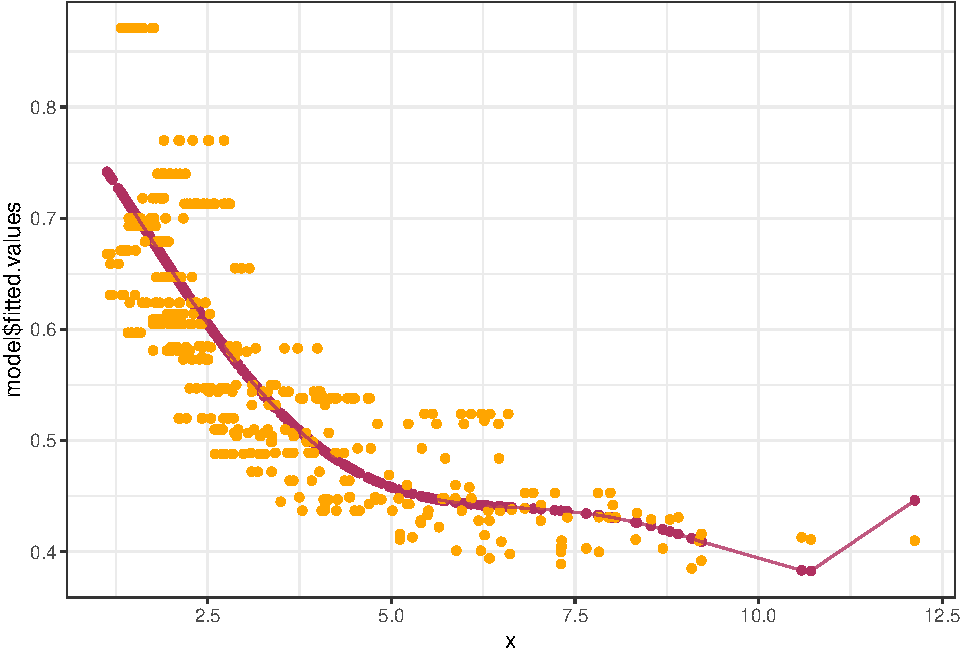
\includegraphics{hw7_files/figure-latex/unnamed-chunk-5-1.pdf}

\begin{Shaded}
\begin{Highlighting}[]
\CommentTok{# Q2: Plot more!}
\NormalTok{RSS =}\StringTok{ }\KeywordTok{c}\NormalTok{()}
\ControlFlowTok{for}\NormalTok{ (i }\ControlFlowTok{in} \DecValTok{1}\OperatorTok{:}\DecValTok{10}\NormalTok{)\{}
\NormalTok{  model <-}\StringTok{ }\KeywordTok{lm}\NormalTok{(y}\OperatorTok{~}\KeywordTok{poly}\NormalTok{(x, }\DataTypeTok{degree =}\NormalTok{ i, }\DataTypeTok{raw =}\NormalTok{ T))}
  \KeywordTok{print}\NormalTok{(}\KeywordTok{ggplot}\NormalTok{() }\OperatorTok{+}\StringTok{ }\KeywordTok{theme_bw}\NormalTok{() }\OperatorTok{+}\StringTok{ }\KeywordTok{geom_point}\NormalTok{(}\KeywordTok{aes}\NormalTok{(}\DataTypeTok{x =}\NormalTok{ x, }\DataTypeTok{y =}\NormalTok{ model}\OperatorTok{$}\NormalTok{fitted.values), }\DataTypeTok{color =} \StringTok{"maroon"}\NormalTok{) }\OperatorTok{+}\StringTok{ }\KeywordTok{geom_point}\NormalTok{(}\KeywordTok{aes}\NormalTok{(}\DataTypeTok{x =}\NormalTok{ x, }\DataTypeTok{y =}\NormalTok{ y), }\DataTypeTok{color =} \StringTok{"orange"}\NormalTok{) }\OperatorTok{+}\StringTok{ }\KeywordTok{geom_line}\NormalTok{(}\KeywordTok{aes}\NormalTok{(}\DataTypeTok{x =}\NormalTok{ x, }\DataTypeTok{y =}\NormalTok{ model}\OperatorTok{$}\NormalTok{fitted.values), }\DataTypeTok{color =} \StringTok{"maroon"}\NormalTok{, }\DataTypeTok{alpha =} \FloatTok{0.8}\NormalTok{) }\OperatorTok{+}\StringTok{ }\KeywordTok{labs}\NormalTok{(}\DataTypeTok{title =} \KeywordTok{paste}\NormalTok{(}\StringTok{"Polynomial Fit with Degree"}\NormalTok{,i, }\DataTypeTok{sep =} \StringTok{" "}\NormalTok{)))}
\NormalTok{  RSS =}\StringTok{ }\KeywordTok{c}\NormalTok{(RSS, }\KeywordTok{sum}\NormalTok{(model}\OperatorTok{$}\NormalTok{residuals}\OperatorTok{^}\DecValTok{2}\NormalTok{))}
  \KeywordTok{print}\NormalTok{(}\KeywordTok{paste}\NormalTok{(}\StringTok{"The RSS of the model with degrees "}\NormalTok{, i, }\StringTok{" is "}\NormalTok{, RSS[i],}\StringTok{"."}\NormalTok{, }\DataTypeTok{sep =} \StringTok{""}\NormalTok{))}
\NormalTok{\}}
\end{Highlighting}
\end{Shaded}

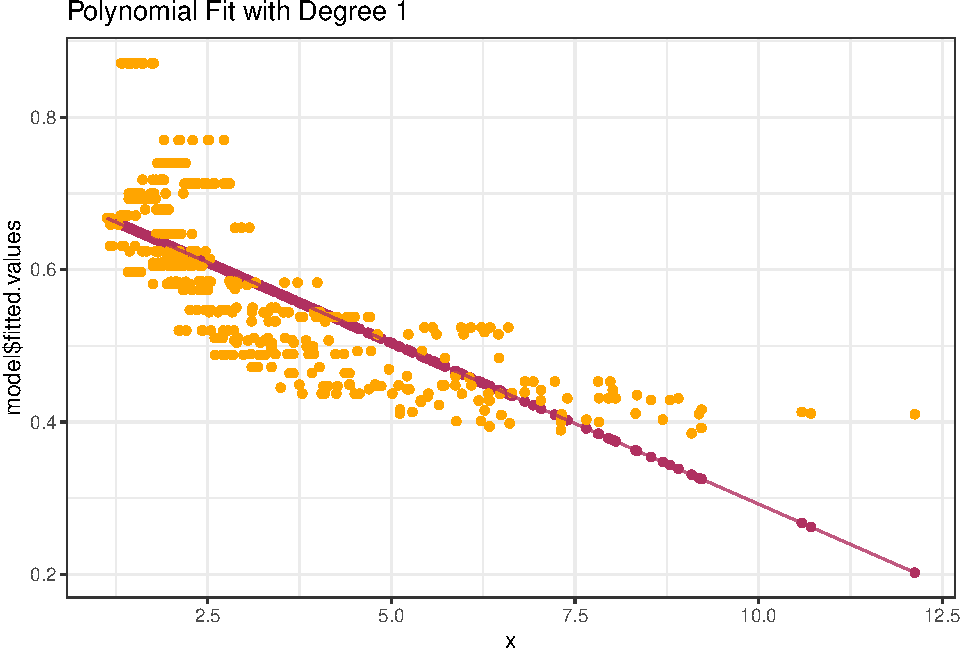
\includegraphics{hw7_files/figure-latex/unnamed-chunk-6-1.pdf}

\begin{verbatim}
## [1] "The RSS of the model with degrees 1 is 2.76856285896928."
\end{verbatim}

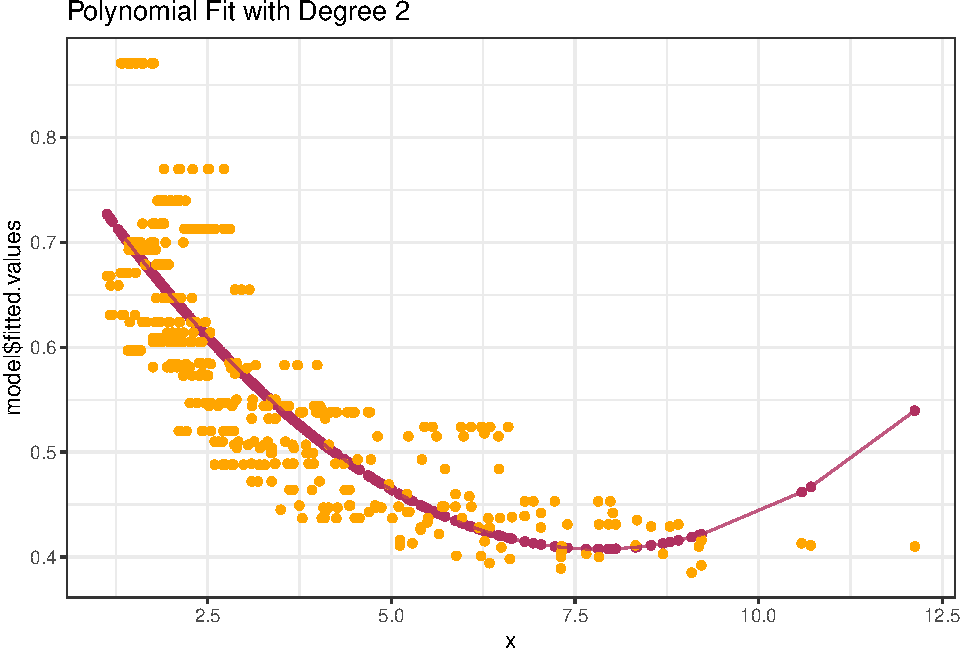
\includegraphics{hw7_files/figure-latex/unnamed-chunk-6-2.pdf}

\begin{verbatim}
## [1] "The RSS of the model with degrees 2 is 2.03526186893526."
\end{verbatim}

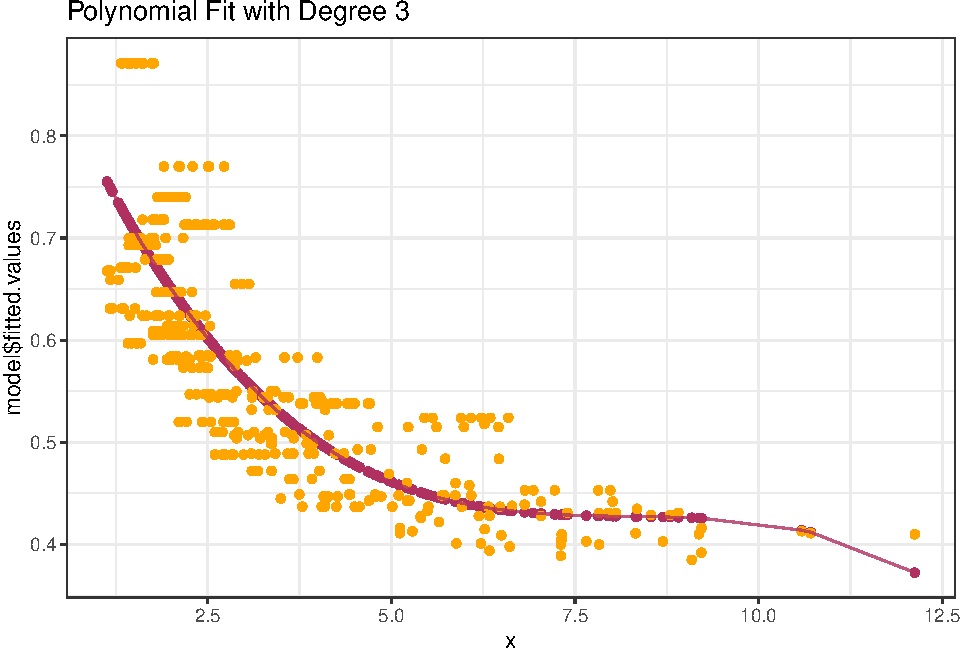
\includegraphics{hw7_files/figure-latex/unnamed-chunk-6-3.pdf}

\begin{verbatim}
## [1] "The RSS of the model with degrees 3 is 1.93410670717907."
\end{verbatim}

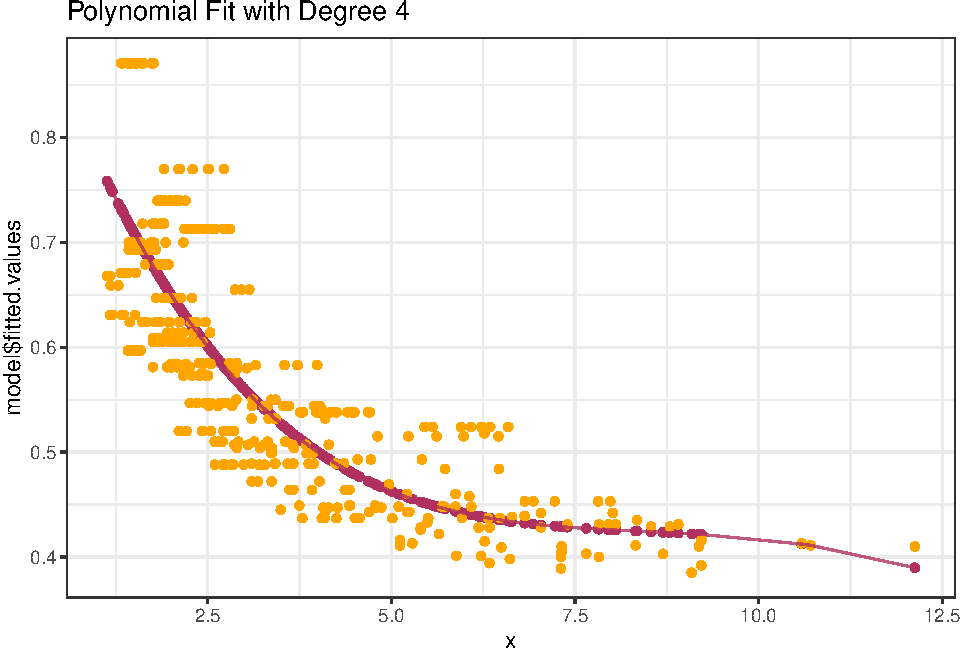
\includegraphics{hw7_files/figure-latex/unnamed-chunk-6-4.pdf}

\begin{verbatim}
## [1] "The RSS of the model with degrees 4 is 1.93298132729859."
\end{verbatim}

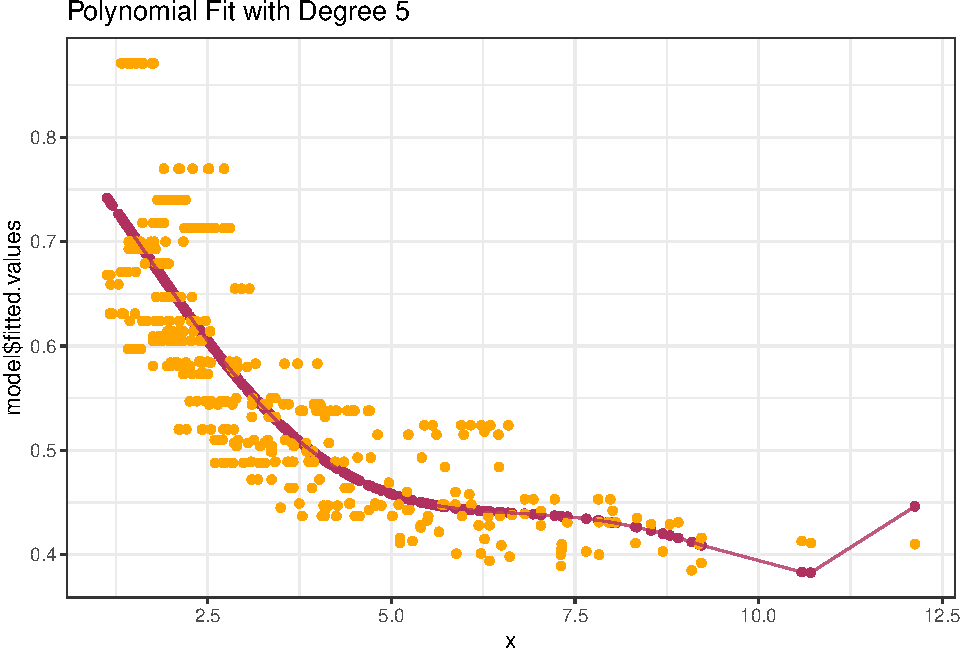
\includegraphics{hw7_files/figure-latex/unnamed-chunk-6-5.pdf}

\begin{verbatim}
## [1] "The RSS of the model with degrees 5 is 1.9152899610843."
\end{verbatim}

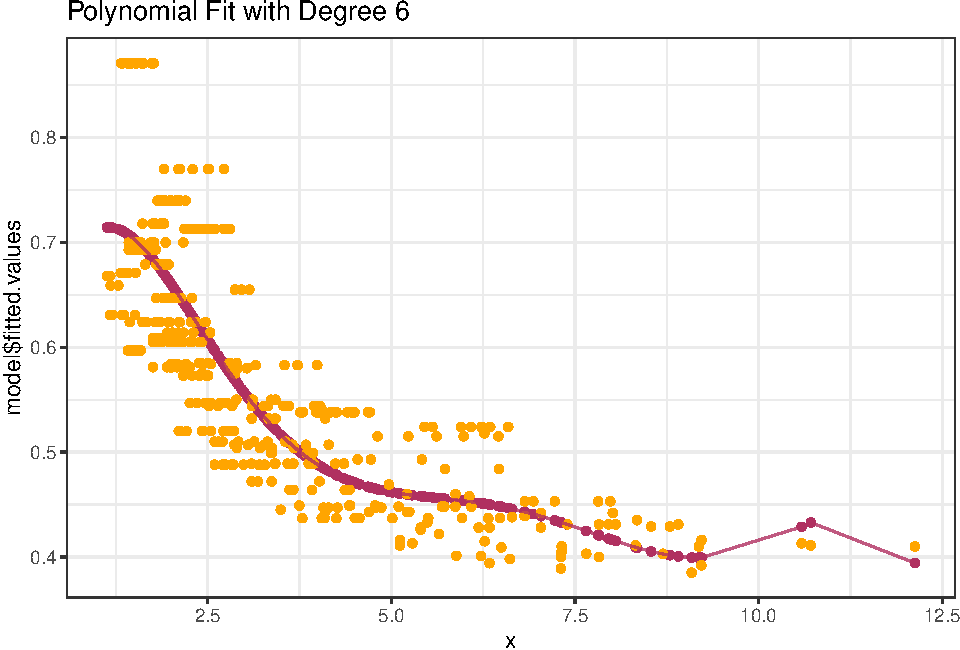
\includegraphics{hw7_files/figure-latex/unnamed-chunk-6-6.pdf}

\begin{verbatim}
## [1] "The RSS of the model with degrees 6 is 1.87825729850817."
\end{verbatim}

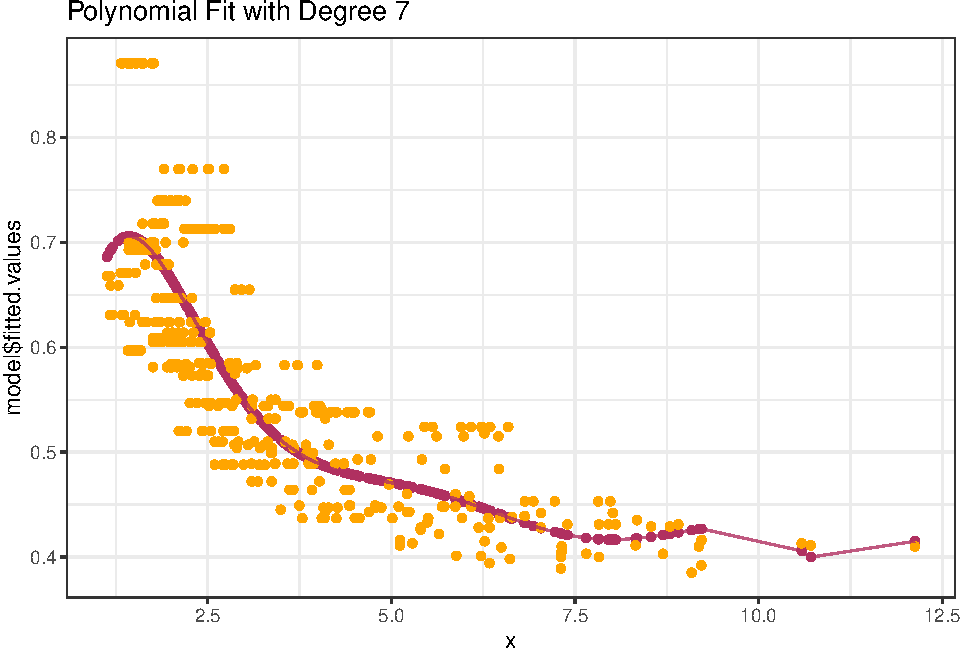
\includegraphics{hw7_files/figure-latex/unnamed-chunk-6-7.pdf}

\begin{verbatim}
## [1] "The RSS of the model with degrees 7 is 1.84948361458297."
\end{verbatim}

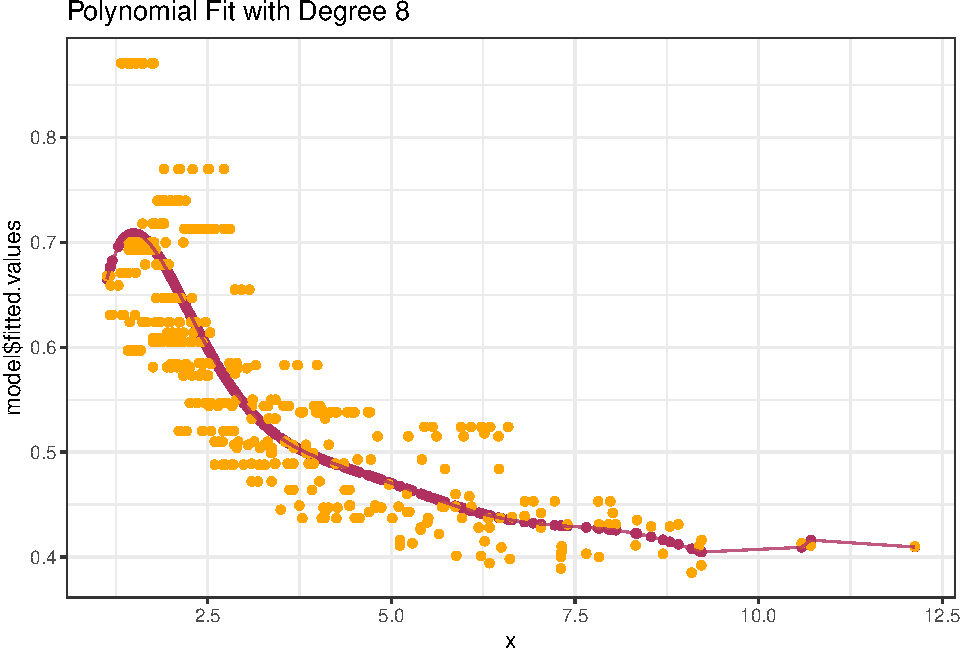
\includegraphics{hw7_files/figure-latex/unnamed-chunk-6-8.pdf}

\begin{verbatim}
## [1] "The RSS of the model with degrees 8 is 1.83562968906761."
\end{verbatim}

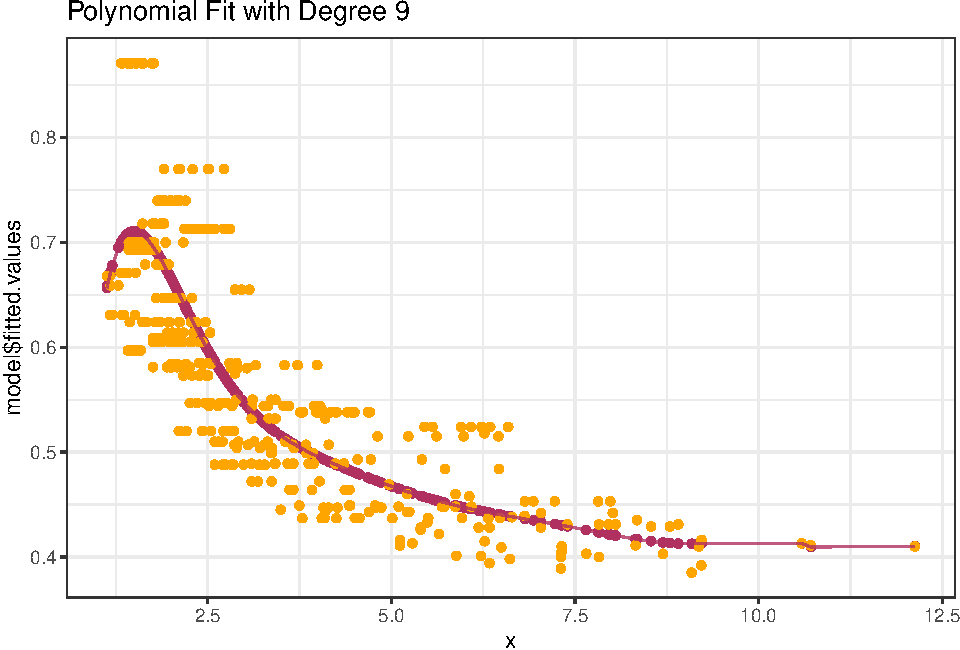
\includegraphics{hw7_files/figure-latex/unnamed-chunk-6-9.pdf}

\begin{verbatim}
## [1] "The RSS of the model with degrees 9 is 1.83333080449161."
\end{verbatim}

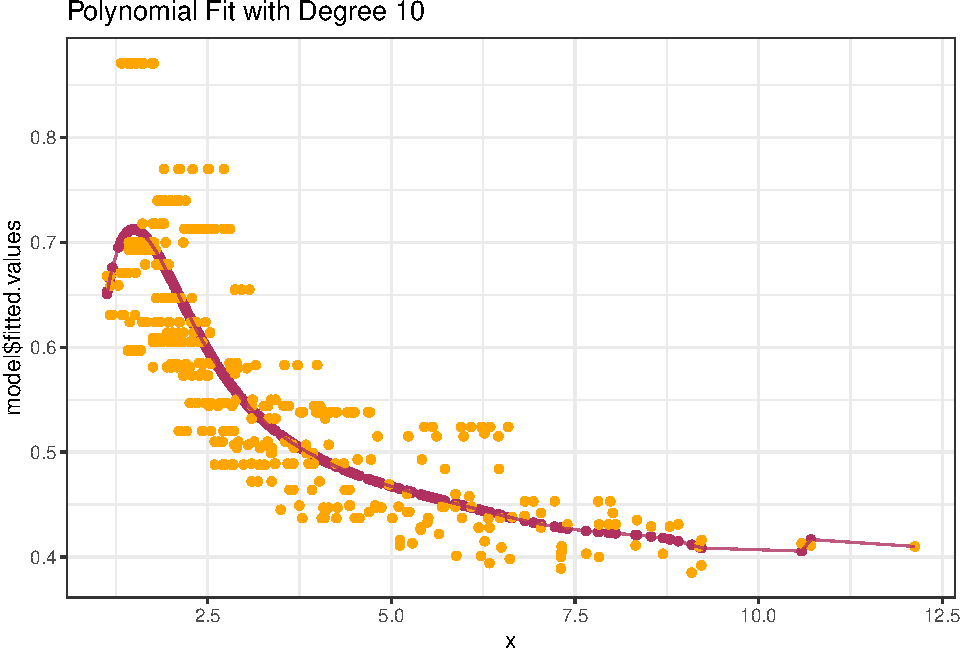
\includegraphics{hw7_files/figure-latex/unnamed-chunk-6-10.pdf}

\begin{verbatim}
## [1] "The RSS of the model with degrees 10 is 1.83217112393014."
\end{verbatim}

\begin{Shaded}
\begin{Highlighting}[]
\KeywordTok{ggplot}\NormalTok{() }\OperatorTok{+}\StringTok{ }\KeywordTok{theme_bw}\NormalTok{() }\OperatorTok{+}\StringTok{ }\KeywordTok{geom_line}\NormalTok{(}\KeywordTok{aes}\NormalTok{(}\DataTypeTok{x =} \DecValTok{1}\OperatorTok{:}\DecValTok{10}\NormalTok{, }\DataTypeTok{y =}\NormalTok{ RSS), }\DataTypeTok{color =} \StringTok{"maroon"}\NormalTok{)}
\end{Highlighting}
\end{Shaded}

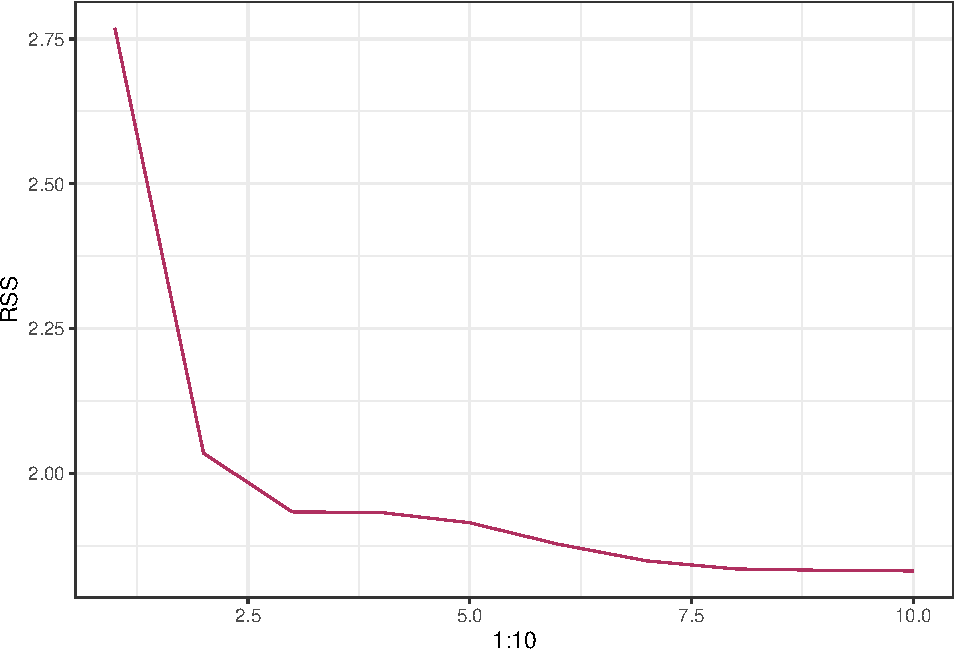
\includegraphics{hw7_files/figure-latex/unnamed-chunk-6-11.pdf}

\begin{Shaded}
\begin{Highlighting}[]
\KeywordTok{set.seed}\NormalTok{(}\DecValTok{11111}\NormalTok{)}
\CommentTok{# Use Cross-Validation}
\NormalTok{trainingSet <-}\StringTok{ }\NormalTok{trainingSet }\OperatorTok
\StringTok{  }\KeywordTok{mutate}\NormalTok{(}\DataTypeTok{instant =} \DecValTok{1}\OperatorTok{:}\KeywordTok{nrow}\NormalTok{(trainingSet), }\DataTypeTok{fold =} \DecValTok{0}\NormalTok{)}
\NormalTok{tempdata <-}\StringTok{ }\NormalTok{trainingSet}

\ControlFlowTok{for}\NormalTok{ (i }\ControlFlowTok{in} \DecValTok{1}\OperatorTok{:}\DecValTok{5}\NormalTok{)\{}
\NormalTok{  num =}\StringTok{ }\DecValTok{100}
  \ControlFlowTok{if}\NormalTok{ (i }\OperatorTok{==}\StringTok{ }\DecValTok{5}\NormalTok{)\{num =}\StringTok{ }\DecValTok{106}\NormalTok{\}}
\NormalTok{  temp <-}\StringTok{  }\KeywordTok{sample_n}\NormalTok{(tempdata, num)}
\NormalTok{  tempdata <-}\StringTok{ }\NormalTok{tempdata }\OperatorTok
\StringTok{    }\KeywordTok{filter}\NormalTok{(}\OperatorTok{!}\NormalTok{(instant }\OperatorTok\StringTok{ }\NormalTok{temp}\OperatorTok{$}\NormalTok{instant))}
\NormalTok{  trainingSet[trainingSet}\OperatorTok{$}\NormalTok{instant }\OperatorTok\StringTok{ }\NormalTok{temp}\OperatorTok{$}\NormalTok{instant,] <-}\StringTok{ }\NormalTok{trainingSet }\OperatorTok
\StringTok{    }\KeywordTok{filter}\NormalTok{(instant }\OperatorTok\StringTok{ }\NormalTok{temp}\OperatorTok{$}\NormalTok{instant) }\OperatorTok
\StringTok{    }\KeywordTok{mutate}\NormalTok{(}\DataTypeTok{fold =}\NormalTok{ i)}
\NormalTok{\}}
\end{Highlighting}
\end{Shaded}

\begin{Shaded}
\begin{Highlighting}[]
\NormalTok{MSE =}\StringTok{ }\KeywordTok{matrix}\NormalTok{(}\DecValTok{0}\NormalTok{, }\DataTypeTok{nrow =} \DecValTok{5}\NormalTok{, }\DataTypeTok{ncol =} \DecValTok{10}\NormalTok{)}
\ControlFlowTok{for}\NormalTok{ (i }\ControlFlowTok{in} \DecValTok{1}\OperatorTok{:}\DecValTok{5}\NormalTok{)\{}
\NormalTok{  train =}\StringTok{ }\NormalTok{trainingSet }\OperatorTok\StringTok{ }\KeywordTok{filter}\NormalTok{(fold }\OperatorTok{!=}\StringTok{ }\NormalTok{i)}
\NormalTok{  test =}\StringTok{ }\NormalTok{trainingSet }\OperatorTok\StringTok{ }\KeywordTok{filter}\NormalTok{(fold }\OperatorTok{==}\StringTok{ }\NormalTok{i)}
  \ControlFlowTok{for}\NormalTok{ (j }\ControlFlowTok{in} \DecValTok{1}\OperatorTok{:}\DecValTok{10}\NormalTok{)\{}
\NormalTok{    model =}\StringTok{ }\KeywordTok{lm}\NormalTok{(nox }\OperatorTok{~}\StringTok{ }\KeywordTok{poly}\NormalTok{(dis, }\DataTypeTok{degree =}\NormalTok{ j, }\DataTypeTok{raw =}\NormalTok{ T), }\DataTypeTok{data =}\NormalTok{ train)}
\NormalTok{    yfit =}\StringTok{ }\KeywordTok{cbind}\NormalTok{(}\DecValTok{1}\NormalTok{, }\KeywordTok{poly}\NormalTok{(test}\OperatorTok{$}\NormalTok{dis, }\DataTypeTok{degree =}\NormalTok{ j, }\DataTypeTok{raw =}\NormalTok{ T)) }\OperatorTok\StringTok{ }\NormalTok{model}\OperatorTok{$}\NormalTok{coefficients}
\NormalTok{    MSE[i,j] =}\StringTok{ }\KeywordTok{mean}\NormalTok{((test}\OperatorTok{$}\NormalTok{nox }\OperatorTok{-}\StringTok{ }\NormalTok{yfit)}\OperatorTok{^}\DecValTok{2}\NormalTok{)}
\NormalTok{  \}}
\NormalTok{\}}
\KeywordTok{which.min}\NormalTok{(}\KeywordTok{apply}\NormalTok{(MSE, }\DecValTok{2}\NormalTok{, mean))}
\end{Highlighting}
\end{Shaded}

\begin{verbatim}
## [1] 3
\end{verbatim}

\begin{Shaded}
\begin{Highlighting}[]
\CommentTok{# The best model is the 3rd degree polynomial}
\KeywordTok{ggplot}\NormalTok{() }\OperatorTok{+}\StringTok{ }\KeywordTok{geom_line}\NormalTok{(}\KeywordTok{aes}\NormalTok{(}\DataTypeTok{x =} \DecValTok{1}\OperatorTok{:}\DecValTok{10}\NormalTok{, }\DataTypeTok{y =} \KeywordTok{apply}\NormalTok{(MSE, }\DecValTok{2}\NormalTok{, mean)), }\DataTypeTok{color =} \StringTok{"maroon"}\NormalTok{) }\OperatorTok{+}\StringTok{ }\KeywordTok{theme_bw}\NormalTok{()}
\end{Highlighting}
\end{Shaded}

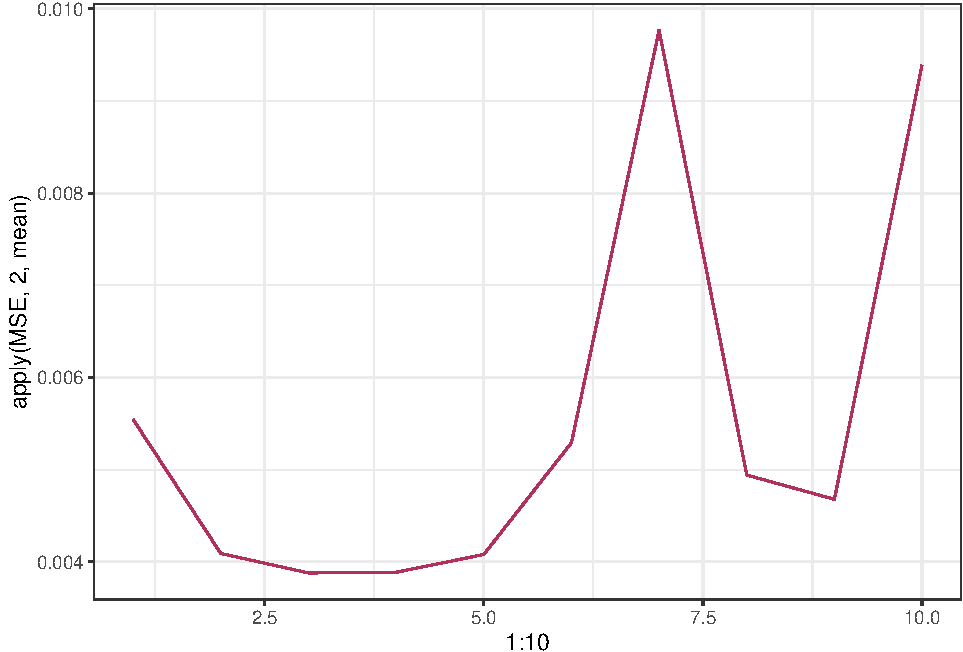
\includegraphics{hw7_files/figure-latex/unnamed-chunk-8-1.pdf}

\begin{Shaded}
\begin{Highlighting}[]
\CommentTok{# The knots are chosen by the quantiles of the data}
\KeywordTok{quantile}\NormalTok{(x)}
\end{Highlighting}
\end{Shaded}

\begin{verbatim}
##        0%       25%       50%       75%      100% 
##  1.129600  2.100175  3.207450  5.188425 12.126500
\end{verbatim}

\begin{Shaded}
\begin{Highlighting}[]
\NormalTok{model <-}\StringTok{ }\KeywordTok{lm}\NormalTok{(nox}\OperatorTok{~}\KeywordTok{bs}\NormalTok{(dis,}\DataTypeTok{knots=}\KeywordTok{c}\NormalTok{(}\FloatTok{2.1}\NormalTok{,}\FloatTok{3.2}\NormalTok{,}\FloatTok{5.2}\NormalTok{)),}\DataTypeTok{data=}\NormalTok{trainingSet)}

\KeywordTok{attach}\NormalTok{(trainingSet)}
\NormalTok{preds=}\KeywordTok{predict}\NormalTok{(model,}\DataTypeTok{newdata=}\KeywordTok{list}\NormalTok{(}\DataTypeTok{dis=}\KeywordTok{seq}\NormalTok{(}\DataTypeTok{from =} \KeywordTok{min}\NormalTok{(dis), }\DataTypeTok{to =} \KeywordTok{max}\NormalTok{(dis))),}\DataTypeTok{se=}\OtherTok{TRUE}\NormalTok{)}

\KeywordTok{plot}\NormalTok{(x, y, }\DataTypeTok{col=}\StringTok{"gray"}\NormalTok{)}
\KeywordTok{lines}\NormalTok{(}\KeywordTok{seq}\NormalTok{(}\DataTypeTok{from =} \KeywordTok{min}\NormalTok{(dis), }\DataTypeTok{to =} \KeywordTok{max}\NormalTok{(dis)),preds}\OperatorTok{$}\NormalTok{fit,}\DataTypeTok{lwd=}\DecValTok{2}\NormalTok{)}
\KeywordTok{lines}\NormalTok{(}\KeywordTok{seq}\NormalTok{(}\DataTypeTok{from =} \KeywordTok{min}\NormalTok{(dis), }\DataTypeTok{to =} \KeywordTok{max}\NormalTok{(dis)),(preds}\OperatorTok{$}\NormalTok{fit }\OperatorTok{+}\DecValTok{2}\OperatorTok{*}\NormalTok{preds}\OperatorTok{$}\NormalTok{se) ,}\DataTypeTok{lty=}\StringTok{"dashed"}\NormalTok{)}
\KeywordTok{lines}\NormalTok{(}\KeywordTok{seq}\NormalTok{(}\DataTypeTok{from =} \KeywordTok{min}\NormalTok{(dis), }\DataTypeTok{to =} \KeywordTok{max}\NormalTok{(dis)),(preds}\OperatorTok{$}\NormalTok{fit }\OperatorTok{-}\DecValTok{2}\OperatorTok{*}\NormalTok{preds}\OperatorTok{$}\NormalTok{se) ,}\DataTypeTok{lty=}\StringTok{"dashed"}\NormalTok{)}
\end{Highlighting}
\end{Shaded}

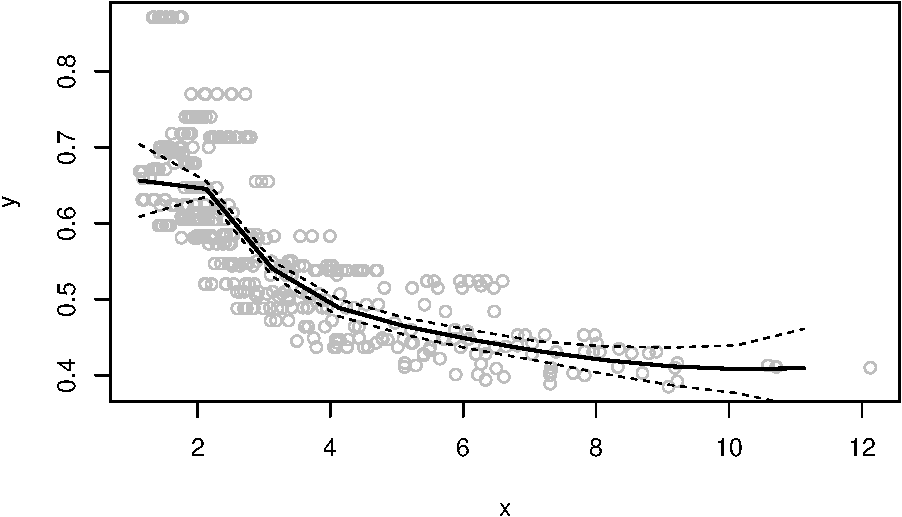
\includegraphics{hw7_files/figure-latex/unnamed-chunk-9-1.pdf}

\begin{Shaded}
\begin{Highlighting}[]
\CommentTok{# Note that in the plot we only choose some sample points, }
\CommentTok{# presenting a broken line instead of a curve}
\ControlFlowTok{for}\NormalTok{ (i }\ControlFlowTok{in} \DecValTok{1}\OperatorTok{:}\DecValTok{10}\NormalTok{)\{}
\NormalTok{  model <-}\StringTok{ }\KeywordTok{lm}\NormalTok{(nox}\OperatorTok{~}\KeywordTok{bs}\NormalTok{(dis,}\DataTypeTok{knots=}\KeywordTok{c}\NormalTok{(}\FloatTok{2.1}\NormalTok{,}\FloatTok{3.2}\NormalTok{,}\FloatTok{5.2}\NormalTok{), }\DataTypeTok{degree =}\NormalTok{ i),}\DataTypeTok{data=}\NormalTok{trainingSet)}
\NormalTok{  preds=}\KeywordTok{predict}\NormalTok{(model,}\DataTypeTok{newdata=}\KeywordTok{list}\NormalTok{(}\DataTypeTok{dis=}\KeywordTok{seq}\NormalTok{(}\DataTypeTok{from =} \KeywordTok{min}\NormalTok{(dis), }\DataTypeTok{to =} \KeywordTok{max}\NormalTok{(dis))),}\DataTypeTok{se=}\OtherTok{TRUE}\NormalTok{)}
  
  \KeywordTok{plot}\NormalTok{(x, y, }\DataTypeTok{col=}\StringTok{"gray"}\NormalTok{)}
  \KeywordTok{lines}\NormalTok{(}\KeywordTok{seq}\NormalTok{(}\DataTypeTok{from =} \KeywordTok{min}\NormalTok{(dis), }\DataTypeTok{to =} \KeywordTok{max}\NormalTok{(dis)),preds}\OperatorTok{$}\NormalTok{fit,}\DataTypeTok{lwd=}\DecValTok{2}\NormalTok{)}
  \KeywordTok{lines}\NormalTok{(}\KeywordTok{seq}\NormalTok{(}\DataTypeTok{from =} \KeywordTok{min}\NormalTok{(dis), }\DataTypeTok{to =} \KeywordTok{max}\NormalTok{(dis)),(preds}\OperatorTok{$}\NormalTok{fit }\OperatorTok{+}\DecValTok{2}\OperatorTok{*}\NormalTok{preds}\OperatorTok{$}\NormalTok{se) ,}\DataTypeTok{lty=}\StringTok{"dashed"}\NormalTok{)}
  \KeywordTok{lines}\NormalTok{(}\KeywordTok{seq}\NormalTok{(}\DataTypeTok{from =} \KeywordTok{min}\NormalTok{(dis), }\DataTypeTok{to =} \KeywordTok{max}\NormalTok{(dis)),(preds}\OperatorTok{$}\NormalTok{fit }\OperatorTok{-}\DecValTok{2}\OperatorTok{*}\NormalTok{preds}\OperatorTok{$}\NormalTok{se) ,}\DataTypeTok{lty=}\StringTok{"dashed"}\NormalTok{)}
  \KeywordTok{title}\NormalTok{(}\KeywordTok{paste}\NormalTok{(}\StringTok{"Spline With Degree "}\NormalTok{, i, }\DataTypeTok{sep =} \StringTok{""}\NormalTok{))}
\NormalTok{\}}
\end{Highlighting}
\end{Shaded}

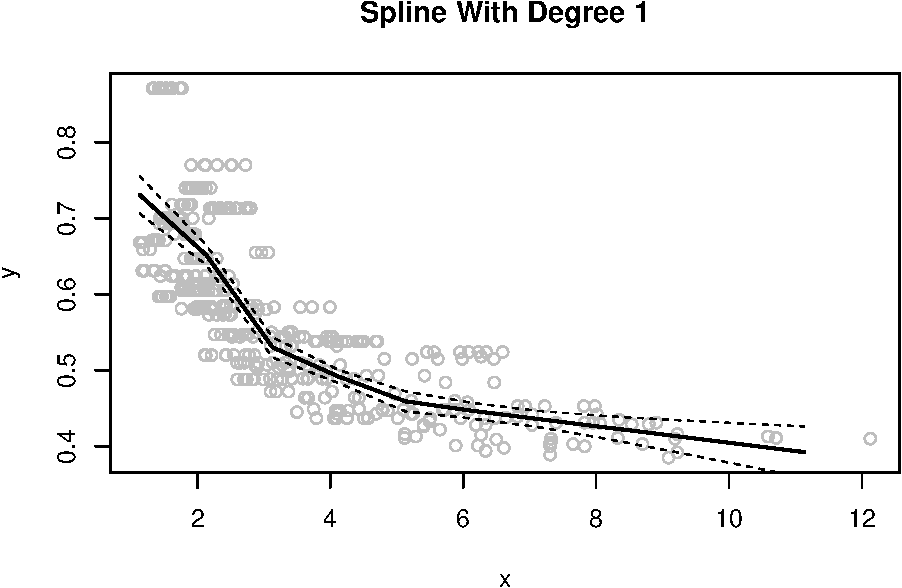
\includegraphics{hw7_files/figure-latex/unnamed-chunk-10-1.pdf}
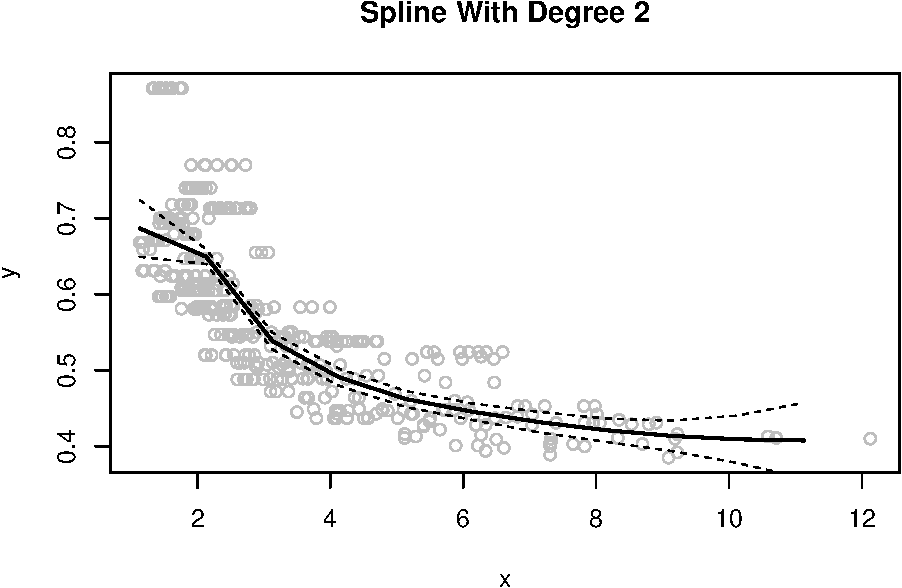
\includegraphics{hw7_files/figure-latex/unnamed-chunk-10-2.pdf}
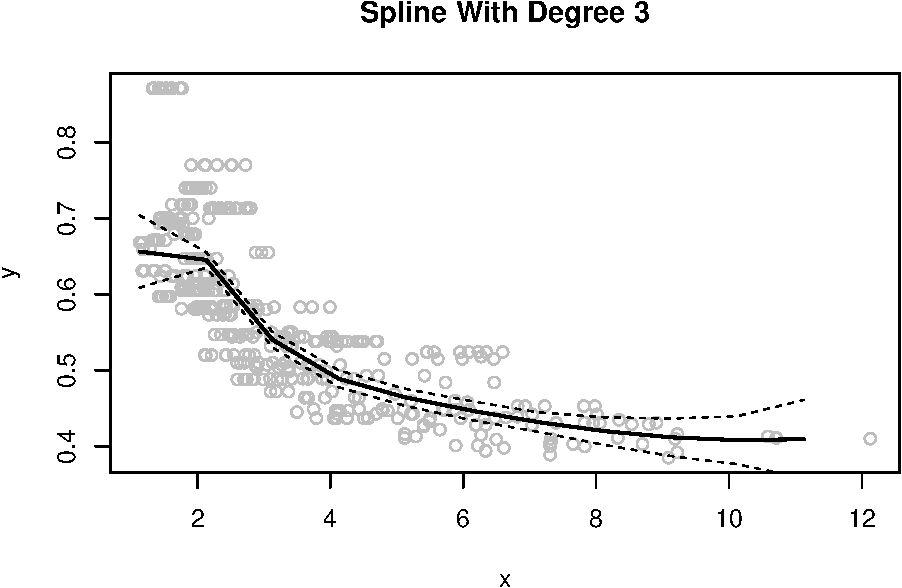
\includegraphics{hw7_files/figure-latex/unnamed-chunk-10-3.pdf}
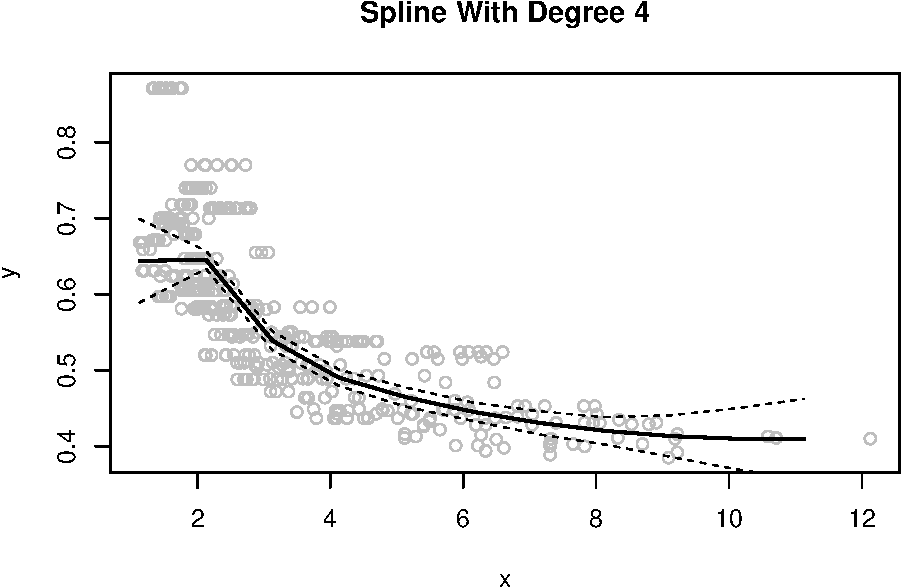
\includegraphics{hw7_files/figure-latex/unnamed-chunk-10-4.pdf}
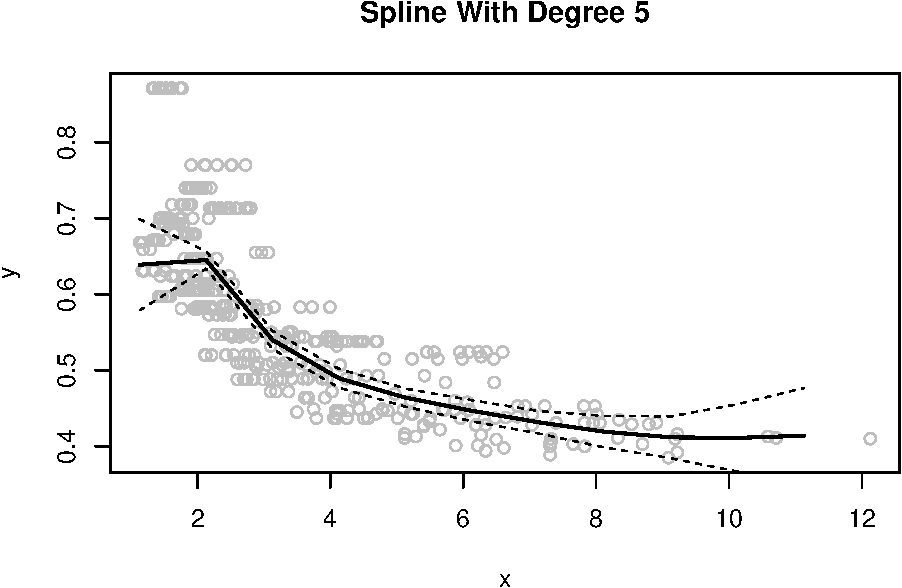
\includegraphics{hw7_files/figure-latex/unnamed-chunk-10-5.pdf}
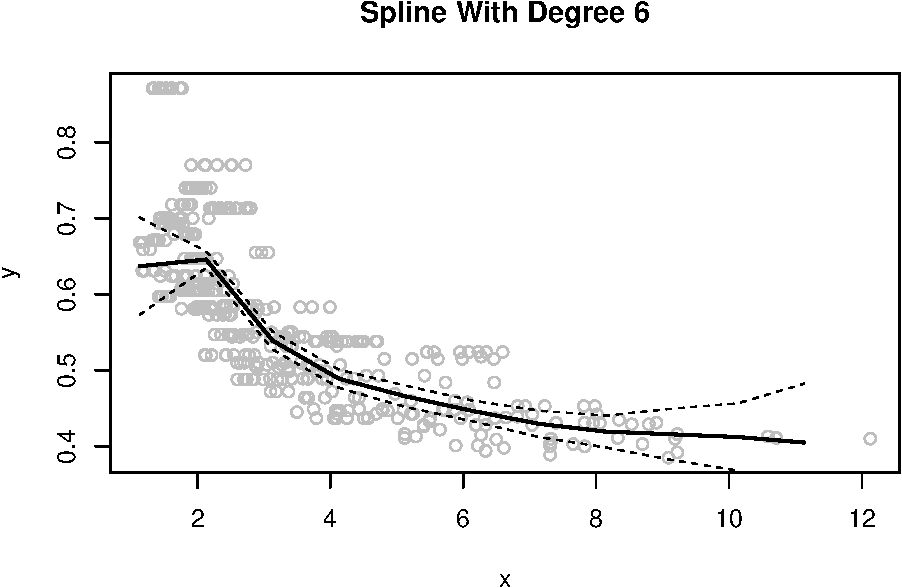
\includegraphics{hw7_files/figure-latex/unnamed-chunk-10-6.pdf}
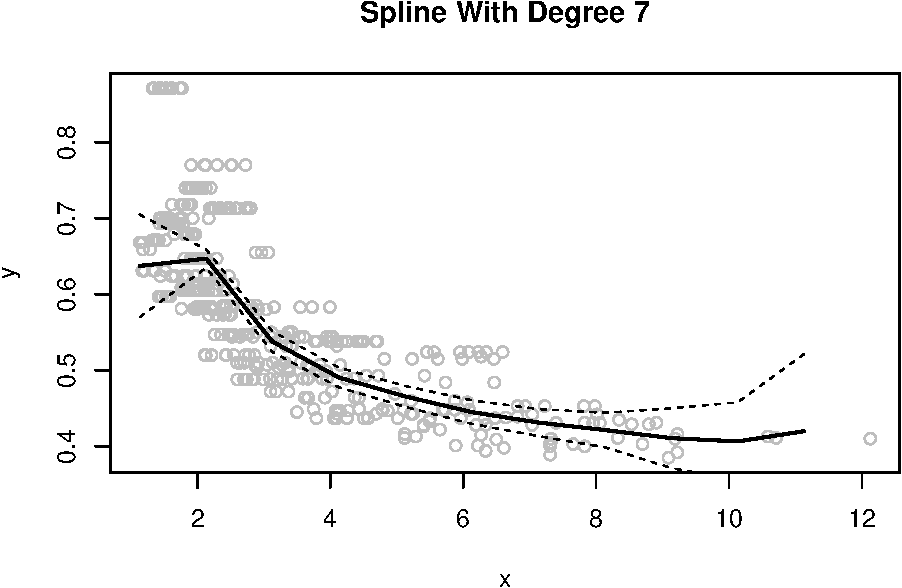
\includegraphics{hw7_files/figure-latex/unnamed-chunk-10-7.pdf}
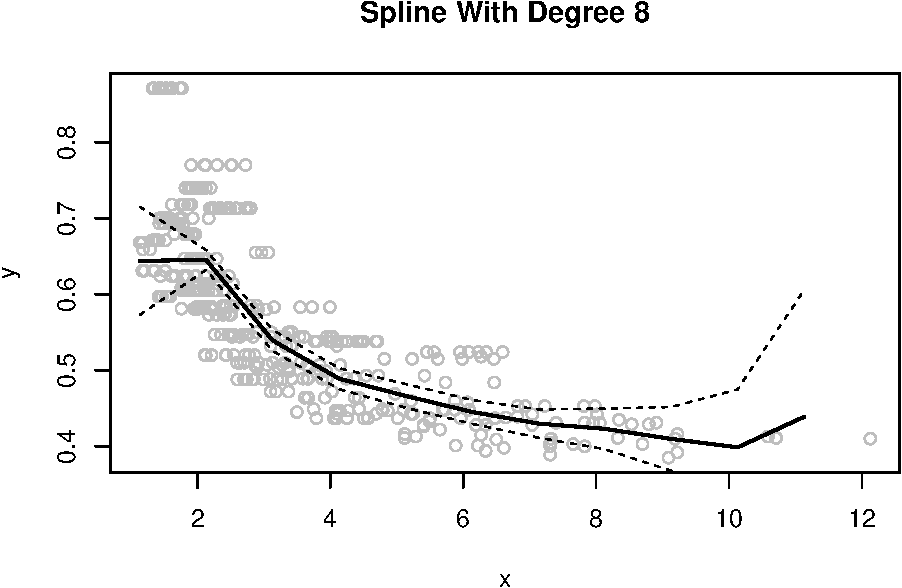
\includegraphics{hw7_files/figure-latex/unnamed-chunk-10-8.pdf}
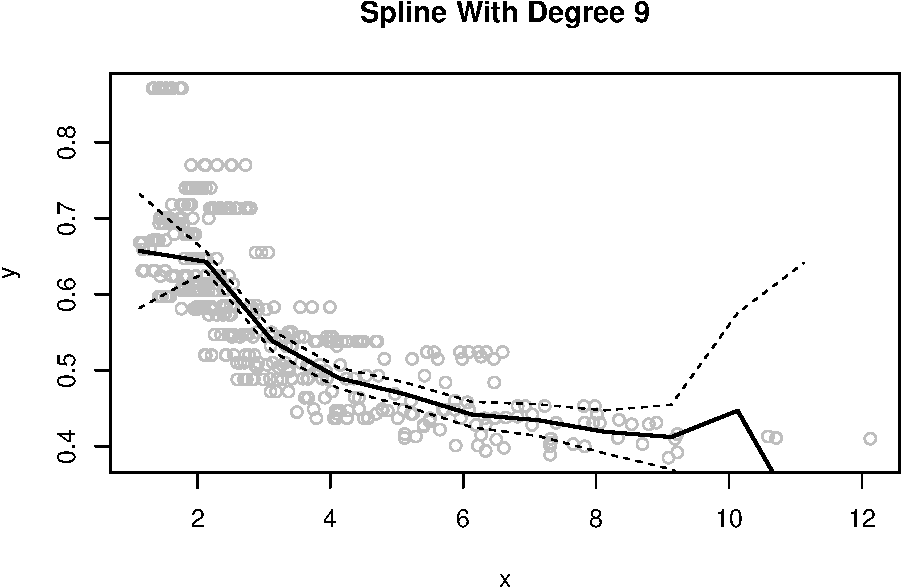
\includegraphics{hw7_files/figure-latex/unnamed-chunk-10-9.pdf}
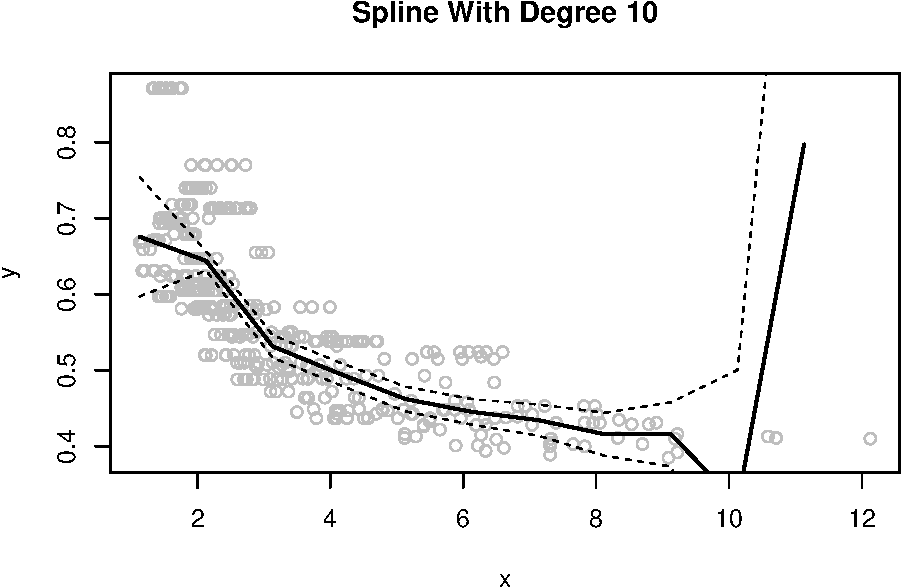
\includegraphics{hw7_files/figure-latex/unnamed-chunk-10-10.pdf}

\begin{Shaded}
\begin{Highlighting}[]
\NormalTok{model <-}\StringTok{ }\KeywordTok{smooth.spline}\NormalTok{(}\DataTypeTok{x =}\NormalTok{ train}\OperatorTok{$}\NormalTok{dis, }\DataTypeTok{y =}\NormalTok{ train}\OperatorTok{$}\NormalTok{nox)}
\NormalTok{temp <-}\StringTok{ }\KeywordTok{predict}\NormalTok{(model, test}\OperatorTok{$}\NormalTok{dis)}
\CommentTok{# Cross-validation}
\NormalTok{MSE =}\StringTok{ }\KeywordTok{matrix}\NormalTok{(}\DecValTok{0}\NormalTok{, }\DataTypeTok{nrow =} \DecValTok{5}\NormalTok{, }\DataTypeTok{ncol =} \DecValTok{9}\NormalTok{)}
\ControlFlowTok{for}\NormalTok{ (i }\ControlFlowTok{in} \DecValTok{1}\OperatorTok{:}\DecValTok{5}\NormalTok{)\{}
\NormalTok{  train =}\StringTok{ }\NormalTok{trainingSet }\OperatorTok\StringTok{ }\KeywordTok{filter}\NormalTok{(fold }\OperatorTok{!=}\StringTok{ }\NormalTok{i)}
\NormalTok{  test =}\StringTok{ }\NormalTok{trainingSet }\OperatorTok\StringTok{ }\KeywordTok{filter}\NormalTok{(fold }\OperatorTok{==}\StringTok{ }\NormalTok{i)}
  \ControlFlowTok{for}\NormalTok{ (j }\ControlFlowTok{in} \DecValTok{2}\OperatorTok{:}\DecValTok{10}\NormalTok{)\{}
\NormalTok{    model <-}\StringTok{ }\KeywordTok{smooth.spline}\NormalTok{(}\DataTypeTok{x =}\NormalTok{ train}\OperatorTok{$}\NormalTok{dis, }\DataTypeTok{y =}\NormalTok{ train}\OperatorTok{$}\NormalTok{nox, }\DataTypeTok{df =}\NormalTok{ j)}
\NormalTok{    yfit =}\StringTok{ }\KeywordTok{predict}\NormalTok{(model, test}\OperatorTok{$}\NormalTok{dis)}\OperatorTok{$}\NormalTok{y}
\NormalTok{    MSE[i,j}\OperatorTok{-}\DecValTok{1}\NormalTok{] =}\StringTok{ }\KeywordTok{mean}\NormalTok{((test}\OperatorTok{$}\NormalTok{nox }\OperatorTok{-}\StringTok{ }\NormalTok{yfit)}\OperatorTok{^}\DecValTok{2}\NormalTok{)}
\NormalTok{  \}}
\NormalTok{\}}
\KeywordTok{which.min}\NormalTok{(}\KeywordTok{apply}\NormalTok{(MSE, }\DecValTok{2}\NormalTok{, mean)) }\OperatorTok{+}\StringTok{ }\DecValTok{1}
\end{Highlighting}
\end{Shaded}

\begin{verbatim}
## [1] 10
\end{verbatim}

\begin{Shaded}
\begin{Highlighting}[]
\CommentTok{# The best model is the 10th degree smooth-spline}
\KeywordTok{ggplot}\NormalTok{() }\OperatorTok{+}\StringTok{ }\KeywordTok{geom_line}\NormalTok{(}\KeywordTok{aes}\NormalTok{(}\DataTypeTok{x =} \DecValTok{2}\OperatorTok{:}\DecValTok{10}\NormalTok{, }\DataTypeTok{y =} \KeywordTok{apply}\NormalTok{(MSE, }\DecValTok{2}\NormalTok{, mean)), }\DataTypeTok{color =} \StringTok{"maroon"}\NormalTok{) }\OperatorTok{+}\StringTok{ }\KeywordTok{theme_bw}\NormalTok{()}
\end{Highlighting}
\end{Shaded}

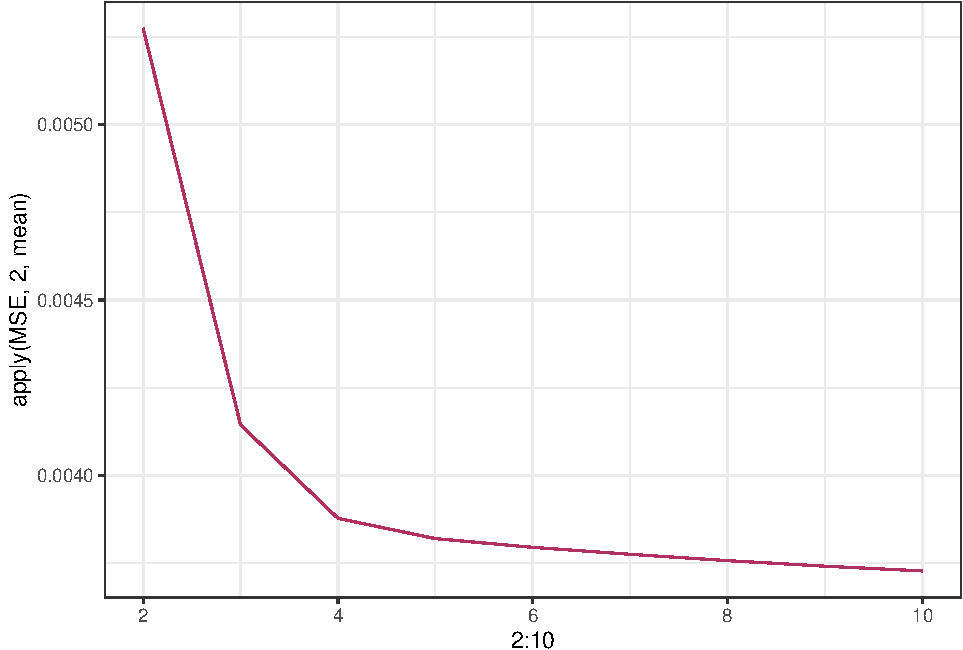
\includegraphics{hw7_files/figure-latex/unnamed-chunk-11-1.pdf}


\end{document}
